\documentclass[twoside]{book}

% Packages required by doxygen
\usepackage{fixltx2e}
\usepackage{calc}
\usepackage{doxygen}
\usepackage[export]{adjustbox} % also loads graphicx
\usepackage{graphicx}
\usepackage[utf8]{inputenc}
\usepackage{makeidx}
\usepackage{multicol}
\usepackage{multirow}
\PassOptionsToPackage{warn}{textcomp}
\usepackage{textcomp}
\usepackage[nointegrals]{wasysym}
\usepackage[table]{xcolor}

% NLS support packages
\usepackage[spanish]{babel}
% Font selection
\usepackage[T1]{fontenc}
\usepackage[scaled=.90]{helvet}
\usepackage{courier}
\usepackage{amssymb}
\usepackage{sectsty}
\renewcommand{\familydefault}{\sfdefault}
\allsectionsfont{%
  \fontseries{bc}\selectfont%
  \color{darkgray}%
}
\renewcommand{\DoxyLabelFont}{%
  \fontseries{bc}\selectfont%
  \color{darkgray}%
}
\newcommand{\+}{\discretionary{\mbox{\scriptsize$\hookleftarrow$}}{}{}}

% Page & text layout
\usepackage{geometry}
\geometry{%
  a4paper,%
  top=2.5cm,%
  bottom=2.5cm,%
  left=2.5cm,%
  right=2.5cm%
}
\tolerance=750
\hfuzz=15pt
\hbadness=750
\setlength{\emergencystretch}{15pt}
\setlength{\parindent}{0cm}
\setlength{\parskip}{3ex plus 2ex minus 2ex}
\makeatletter
\renewcommand{\paragraph}{%
  \@startsection{paragraph}{4}{0ex}{-1.0ex}{1.0ex}{%
    \normalfont\normalsize\bfseries\SS@parafont%
  }%
}
\renewcommand{\subparagraph}{%
  \@startsection{subparagraph}{5}{0ex}{-1.0ex}{1.0ex}{%
    \normalfont\normalsize\bfseries\SS@subparafont%
  }%
}
\makeatother

% Headers & footers
\usepackage{fancyhdr}
\pagestyle{fancyplain}
\fancyhead[LE]{\fancyplain{}{\bfseries\thepage}}
\fancyhead[CE]{\fancyplain{}{}}
\fancyhead[RE]{\fancyplain{}{\bfseries\leftmark}}
\fancyhead[LO]{\fancyplain{}{\bfseries\rightmark}}
\fancyhead[CO]{\fancyplain{}{}}
\fancyhead[RO]{\fancyplain{}{\bfseries\thepage}}
\fancyfoot[LE]{\fancyplain{}{}}
\fancyfoot[CE]{\fancyplain{}{}}
\fancyfoot[RE]{\fancyplain{}{\bfseries\scriptsize Generado por Doxygen }}
\fancyfoot[LO]{\fancyplain{}{\bfseries\scriptsize Generado por Doxygen }}
\fancyfoot[CO]{\fancyplain{}{}}
\fancyfoot[RO]{\fancyplain{}{}}
\renewcommand{\footrulewidth}{0.4pt}
\renewcommand{\chaptermark}[1]{%
  \markboth{#1}{}%
}
\renewcommand{\sectionmark}[1]{%
  \markright{\thesection\ #1}%
}

% Indices & bibliography
\usepackage{natbib}
\usepackage[titles]{tocloft}
\setcounter{tocdepth}{3}
\setcounter{secnumdepth}{5}
\makeindex

% Hyperlinks (required, but should be loaded last)
\usepackage{ifpdf}
\ifpdf
  \usepackage[pdftex,pagebackref=true]{hyperref}
\else
  \usepackage[ps2pdf,pagebackref=true]{hyperref}
\fi
\hypersetup{%
  colorlinks=true,%
  linkcolor=blue,%
  citecolor=blue,%
  unicode%
}

% Custom commands
\newcommand{\clearemptydoublepage}{%
  \newpage{\pagestyle{empty}\cleardoublepage}%
}

\usepackage{caption}
\captionsetup{labelsep=space,justification=centering,font={bf},singlelinecheck=off,skip=4pt,position=top}

%===== C O N T E N T S =====

\begin{document}

% Titlepage & ToC
\hypersetup{pageanchor=false,
             bookmarksnumbered=true,
             pdfencoding=unicode
            }
\pagenumbering{roman}
\begin{titlepage}
\vspace*{7cm}
\begin{center}%
{\Large Practica 2 }\\
\vspace*{1cm}
{\large Generado por Doxygen 1.8.11}\\
\end{center}
\end{titlepage}
\clearemptydoublepage
\tableofcontents
\clearemptydoublepage
\pagenumbering{arabic}
\hypersetup{pageanchor=true}

%--- Begin generated contents ---
\chapter{Índice de clases}
\section{Lista de clases}
Lista de las clases, estructuras, uniones e interfaces con una breve descripción\+:\begin{DoxyCompactList}
\item\contentsline{section}{\hyperlink{struct__Apuesta}{\+\_\+\+Apuesta} \\*Estructura apuesta }{\pageref{struct__Apuesta}}{}
\item\contentsline{section}{\hyperlink{struct__Caballo}{\+\_\+\+Caballo} \\*Estructura caballo }{\pageref{struct__Caballo}}{}
\item\contentsline{section}{\hyperlink{struct__Carrera}{\+\_\+\+Carrera} \\*Estructura carrera }{\pageref{struct__Carrera}}{}
\item\contentsline{section}{\hyperlink{struct__Mensaje}{\+\_\+\+Mensaje} \\*Estructura mensaje que contiene todos sus parametros necesarios para la realización del ejercicio con colas de mensajes }{\pageref{struct__Mensaje}}{}
\item\contentsline{section}{\hyperlink{struct__Monitor}{\+\_\+\+Monitor} \\*Estructura monitor }{\pageref{struct__Monitor}}{}
\item\contentsline{section}{\hyperlink{struct__Ventanilla}{\+\_\+\+Ventanilla} \\*Estructura ventanilla }{\pageref{struct__Ventanilla}}{}
\end{DoxyCompactList}

\chapter{Indice de archivos}
\section{Lista de archivos}
Lista de todos los archivos documentados y con descripciones breves\+:\begin{DoxyCompactList}
\item\contentsline{section}{\hyperlink{ejercicio10_8c}{ejercicio10.\+c} \\*Implementa el ejercicio 10 de mascaras }{\pageref{ejercicio10_8c}}{}
\item\contentsline{section}{\hyperlink{ejercicio3a_8c}{ejercicio3a.\+c} \\*Implementa el ejercicio 3a de procesos con un solo padre }{\pageref{ejercicio3a_8c}}{}
\item\contentsline{section}{\hyperlink{ejercicio3b_8c}{ejercicio3b.\+c} \\*Implementa el ejercicio 3b de hilos de un proceso }{\pageref{ejercicio3b_8c}}{}
\item\contentsline{section}{\hyperlink{ejercicio4a_8c}{ejercicio4a.\+c} \\*Implementa el ejercicio 4a de multiplicacion de matrices }{\pageref{ejercicio4a_8c}}{}
\item\contentsline{section}{\hyperlink{ejercicio4b_8c}{ejercicio4b.\+c} \\*Implementa el ejercicio 4b de multiplicacion de matrices }{\pageref{ejercicio4b_8c}}{}
\item\contentsline{section}{\hyperlink{ejercicio6_8c}{ejercicio6.\+c} \\*Implementa el ejercicio 6 de señales }{\pageref{ejercicio6_8c}}{}
\end{DoxyCompactList}

\chapter{Documentación de las clases}
\hypertarget{struct__params}{}\section{Referencia de la Estructura \+\_\+params}
\label{struct__params}\index{\+\_\+params@{\+\_\+params}}


Estructura params que contiene los parametros necesarios para que el hilo multiplique un matriz por un numero entero.  




Diagrama de colaboración para \+\_\+params\+:\nopagebreak
\begin{figure}[H]
\begin{center}
\leavevmode
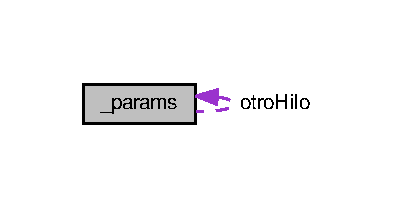
\includegraphics[width=189pt]{struct__params__coll__graph}
\end{center}
\end{figure}
\subsection*{Atributos públicos}
\begin{DoxyCompactItemize}
\item 
int \hyperlink{struct__params_aecffef63bfeb1c33b37bd5df12a98401}{dim}
\item 
int \hyperlink{struct__params_a142e538b8c88b8748ad390b6a86fe17d}{multiplicador}
\item 
int $\ast$ \hyperlink{struct__params_a04b3f21e1f7c21b17a510c2a4ee0e552}{matriz}
\item 
int \hyperlink{struct__params_a160a4d501715e51cfa0a2f289b6c5b14}{nhilo}
\item 
int \hyperlink{struct__params_a8ebf07d62261f18feb39cad26d027616}{fila}
\item 
struct \hyperlink{struct__params}{\+\_\+params} $\ast$ \hyperlink{struct__params_a21ba0961d6fcfa8c876ba58142d181be}{otro\+Hilo}
\end{DoxyCompactItemize}


\subsection{Descripción detallada}
Estructura params que contiene los parametros necesarios para que el hilo multiplique un matriz por un numero entero. 

Estructura params que contiene los parametros necesarios para que el hilo multiplique un matriz por un numero entero. Se ha incluido un puntero a la propia estructura que apuntara a la estructura del otro hilo. 

\subsection{Documentación de los datos miembro}
\index{\+\_\+params@{\+\_\+params}!dim@{dim}}
\index{dim@{dim}!\+\_\+params@{\+\_\+params}}
\subsubsection[{\texorpdfstring{dim}{dim}}]{\setlength{\rightskip}{0pt plus 5cm}int \+\_\+params\+::dim}\hypertarget{struct__params_aecffef63bfeb1c33b37bd5df12a98401}{}\label{struct__params_aecffef63bfeb1c33b37bd5df12a98401}
Dimension matriz \index{\+\_\+params@{\+\_\+params}!fila@{fila}}
\index{fila@{fila}!\+\_\+params@{\+\_\+params}}
\subsubsection[{\texorpdfstring{fila}{fila}}]{\setlength{\rightskip}{0pt plus 5cm}int \+\_\+params\+::fila}\hypertarget{struct__params_a8ebf07d62261f18feb39cad26d027616}{}\label{struct__params_a8ebf07d62261f18feb39cad26d027616}
Identificador de fila \index{\+\_\+params@{\+\_\+params}!matriz@{matriz}}
\index{matriz@{matriz}!\+\_\+params@{\+\_\+params}}
\subsubsection[{\texorpdfstring{matriz}{matriz}}]{\setlength{\rightskip}{0pt plus 5cm}int $\ast$ \+\_\+params\+::matriz}\hypertarget{struct__params_a04b3f21e1f7c21b17a510c2a4ee0e552}{}\label{struct__params_a04b3f21e1f7c21b17a510c2a4ee0e552}
Matriz \index{\+\_\+params@{\+\_\+params}!multiplicador@{multiplicador}}
\index{multiplicador@{multiplicador}!\+\_\+params@{\+\_\+params}}
\subsubsection[{\texorpdfstring{multiplicador}{multiplicador}}]{\setlength{\rightskip}{0pt plus 5cm}int \+\_\+params\+::multiplicador}\hypertarget{struct__params_a142e538b8c88b8748ad390b6a86fe17d}{}\label{struct__params_a142e538b8c88b8748ad390b6a86fe17d}
Escalar \index{\+\_\+params@{\+\_\+params}!nhilo@{nhilo}}
\index{nhilo@{nhilo}!\+\_\+params@{\+\_\+params}}
\subsubsection[{\texorpdfstring{nhilo}{nhilo}}]{\setlength{\rightskip}{0pt plus 5cm}int \+\_\+params\+::nhilo}\hypertarget{struct__params_a160a4d501715e51cfa0a2f289b6c5b14}{}\label{struct__params_a160a4d501715e51cfa0a2f289b6c5b14}
Identificador del hilo \index{\+\_\+params@{\+\_\+params}!otro\+Hilo@{otro\+Hilo}}
\index{otro\+Hilo@{otro\+Hilo}!\+\_\+params@{\+\_\+params}}
\subsubsection[{\texorpdfstring{otro\+Hilo}{otroHilo}}]{\setlength{\rightskip}{0pt plus 5cm}struct {\bf \+\_\+params}$\ast$ \+\_\+params\+::otro\+Hilo}\hypertarget{struct__params_a21ba0961d6fcfa8c876ba58142d181be}{}\label{struct__params_a21ba0961d6fcfa8c876ba58142d181be}
Estructura del otro hilo 

La documentación para esta estructura fue generada a partir de los siguientes ficheros\+:\begin{DoxyCompactItemize}
\item 
\hyperlink{ejercicio4a_8c}{ejercicio4a.\+c}\item 
\hyperlink{ejercicio4b_8c}{ejercicio4b.\+c}\end{DoxyCompactItemize}

\chapter{Documentación de archivos}
\hypertarget{ejercicio10_8c}{}\section{Referencia del Archivo ejercicio10.\+c}
\label{ejercicio10_8c}\index{ejercicio10.\+c@{ejercicio10.\+c}}


Implementa el ejercicio 10 de mascaras.  


{\ttfamily \#include $<$stdio.\+h$>$}\\*
{\ttfamily \#include $<$stdlib.\+h$>$}\\*
{\ttfamily \#include $<$string.\+h$>$}\\*
{\ttfamily \#include $<$signal.\+h$>$}\\*
{\ttfamily \#include $<$time.\+h$>$}\\*
{\ttfamily \#include $<$sys/types.\+h$>$}\\*
{\ttfamily \#include $<$sys/wait.\+h$>$}\\*
{\ttfamily \#include $<$unistd.\+h$>$}\\*
Dependencia gráfica adjunta para ejercicio10.\+c\+:\nopagebreak
\begin{figure}[H]
\begin{center}
\leavevmode
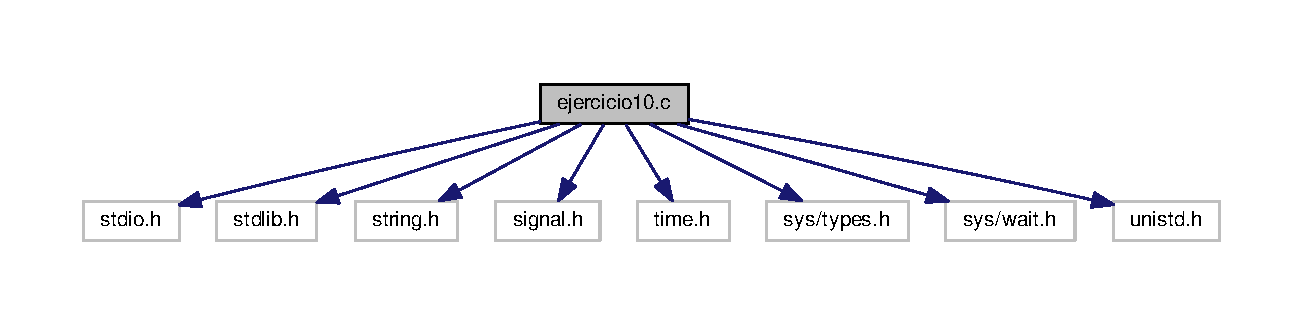
\includegraphics[width=350pt]{ejercicio10_8c__incl}
\end{center}
\end{figure}
\subsection*{\textquotesingle{}defines\textquotesingle{}}
\begin{DoxyCompactItemize}
\item 
\#define {\bfseries N\+U\+M\+P\+A\+L\+A\+B\+R\+AS}~13\hypertarget{ejercicio10_8c_a2b79500034922417daea33a4a20e4546}{}\label{ejercicio10_8c_a2b79500034922417daea33a4a20e4546}

\end{DoxyCompactItemize}
\subsection*{Funciones}
\begin{DoxyCompactItemize}
\item 
void {\bfseries captura} (int sig)\hypertarget{ejercicio10_8c_a9f37a0f7ce38c68b8193b279dff1226b}{}\label{ejercicio10_8c_a9f37a0f7ce38c68b8193b279dff1226b}

\item 
int \hyperlink{ejercicio10_8c_ae66f6b31b5ad750f1fe042a706a4e3d4}{main} ()
\begin{DoxyCompactList}\small\item\em funcion de procesos con un solo padre \end{DoxyCompactList}\end{DoxyCompactItemize}


\subsection{Descripción detallada}
Implementa el ejercicio 10 de mascaras. 

\begin{DoxyAuthor}{Autor}
Andres Salas \href{mailto:andres.salas@estudiante.uam.es}{\tt andres.\+salas@estudiante.\+uam.\+es} 

Antonio Martin \href{mailto:antonio.martinmasuda@estudiante.uam.es}{\tt antonio.\+martinmasuda@estudiante.\+uam.\+es} 
\end{DoxyAuthor}
\begin{DoxyNote}{Nota}
Grupo 2202 
\end{DoxyNote}
\begin{DoxyVersion}{Versión}
1.\+0 
\end{DoxyVersion}
\begin{DoxyDate}{Fecha}
11/03/2017 
\end{DoxyDate}


\subsection{Documentación de las funciones}
\index{ejercicio10.\+c@{ejercicio10.\+c}!main@{main}}
\index{main@{main}!ejercicio10.\+c@{ejercicio10.\+c}}
\subsubsection[{\texorpdfstring{main()}{main()}}]{\setlength{\rightskip}{0pt plus 5cm}int main (
\begin{DoxyParamCaption}
{}
\end{DoxyParamCaption}
)}\hypertarget{ejercicio10_8c_ae66f6b31b5ad750f1fe042a706a4e3d4}{}\label{ejercicio10_8c_ae66f6b31b5ad750f1fe042a706a4e3d4}


funcion de procesos con un solo padre 

\begin{DoxyReturn}{Devuelve}
int\+: valor de exito o fracaso 
\end{DoxyReturn}

\hypertarget{ejercicio3a_8c}{}\section{Referencia del Archivo ejercicio3a.\+c}
\label{ejercicio3a_8c}\index{ejercicio3a.\+c@{ejercicio3a.\+c}}


Implementa el ejercicio 3a de procesos con un solo padre.  


{\ttfamily \#include $<$stdio.\+h$>$}\\*
{\ttfamily \#include $<$stdlib.\+h$>$}\\*
{\ttfamily \#include $<$sys/types.\+h$>$}\\*
{\ttfamily \#include $<$sys/wait.\+h$>$}\\*
{\ttfamily \#include $<$sys/time.\+h$>$}\\*
{\ttfamily \#include $<$unistd.\+h$>$}\\*
Dependencia gráfica adjunta para ejercicio3a.\+c\+:\nopagebreak
\begin{figure}[H]
\begin{center}
\leavevmode
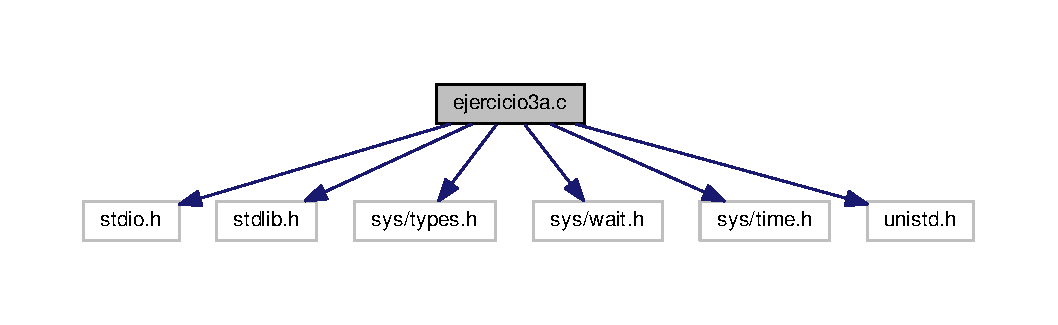
\includegraphics[width=350pt]{ejercicio3a_8c__incl}
\end{center}
\end{figure}
\subsection*{\textquotesingle{}defines\textquotesingle{}}
\begin{DoxyCompactItemize}
\item 
\#define \hyperlink{ejercicio3a_8c_acee2369f62e4a096d243dec3cd7d0b00}{N\+U\+M\+\_\+\+P\+R\+OC}~100
\end{DoxyCompactItemize}
\subsection*{Funciones}
\begin{DoxyCompactItemize}
\item 
int $\ast$ \hyperlink{ejercicio3a_8c_af7397f188966cc18c1be25c8dad77bcb}{is\+\_\+prime} (int np)
\begin{DoxyCompactList}\small\item\em funcion que lista los np primeros primos \end{DoxyCompactList}\item 
int \hyperlink{ejercicio3a_8c_a0ddf1224851353fc92bfbff6f499fa97}{main} (int argc, char $\ast$argv\mbox{[}$\,$\mbox{]})
\begin{DoxyCompactList}\small\item\em funcion de procesos con un solo padre \end{DoxyCompactList}\end{DoxyCompactItemize}


\subsection{Descripción detallada}
Implementa el ejercicio 3a de procesos con un solo padre. 

\begin{DoxyAuthor}{Autor}
Andres Salas \href{mailto:andres.salas@estudiante.uam.es}{\tt andres.\+salas@estudiante.\+uam.\+es} 

Antonio Martin \href{mailto:antonio.martinmasuda@estudiante.uam.es}{\tt antonio.\+martinmasuda@estudiante.\+uam.\+es} 
\end{DoxyAuthor}
\begin{DoxyNote}{Nota}
Grupo 2202 
\end{DoxyNote}
\begin{DoxyVersion}{Versión}
1.\+0 
\end{DoxyVersion}
\begin{DoxyDate}{Fecha}
03/03/2017 
\end{DoxyDate}


\subsection{Documentación de los \textquotesingle{}defines\textquotesingle{}}
\index{ejercicio3a.\+c@{ejercicio3a.\+c}!N\+U\+M\+\_\+\+P\+R\+OC@{N\+U\+M\+\_\+\+P\+R\+OC}}
\index{N\+U\+M\+\_\+\+P\+R\+OC@{N\+U\+M\+\_\+\+P\+R\+OC}!ejercicio3a.\+c@{ejercicio3a.\+c}}
\subsubsection[{\texorpdfstring{N\+U\+M\+\_\+\+P\+R\+OC}{NUM_PROC}}]{\setlength{\rightskip}{0pt plus 5cm}\#define N\+U\+M\+\_\+\+P\+R\+OC~100}\hypertarget{ejercicio3a_8c_acee2369f62e4a096d243dec3cd7d0b00}{}\label{ejercicio3a_8c_acee2369f62e4a096d243dec3cd7d0b00}
Numero de procesos del bucle for 

\subsection{Documentación de las funciones}
\index{ejercicio3a.\+c@{ejercicio3a.\+c}!is\+\_\+prime@{is\+\_\+prime}}
\index{is\+\_\+prime@{is\+\_\+prime}!ejercicio3a.\+c@{ejercicio3a.\+c}}
\subsubsection[{\texorpdfstring{is\+\_\+prime(int np)}{is_prime(int np)}}]{\setlength{\rightskip}{0pt plus 5cm}int$\ast$ is\+\_\+prime (
\begin{DoxyParamCaption}
\item[{int}]{np}
\end{DoxyParamCaption}
)}\hypertarget{ejercicio3a_8c_af7397f188966cc18c1be25c8dad77bcb}{}\label{ejercicio3a_8c_af7397f188966cc18c1be25c8dad77bcb}


funcion que lista los np primeros primos 


\begin{DoxyParams}{Parámetros}
{\em np} & numero de primos a calcular \\
\hline
\end{DoxyParams}
\begin{DoxyReturn}{Devuelve}
int\+: valor de exito o fracaso 
\end{DoxyReturn}
\index{ejercicio3a.\+c@{ejercicio3a.\+c}!main@{main}}
\index{main@{main}!ejercicio3a.\+c@{ejercicio3a.\+c}}
\subsubsection[{\texorpdfstring{main(int argc, char $\ast$argv[])}{main(int argc, char *argv[])}}]{\setlength{\rightskip}{0pt plus 5cm}int main (
\begin{DoxyParamCaption}
\item[{int}]{argc, }
\item[{char $\ast$}]{argv\mbox{[}$\,$\mbox{]}}
\end{DoxyParamCaption}
)}\hypertarget{ejercicio3a_8c_a0ddf1224851353fc92bfbff6f499fa97}{}\label{ejercicio3a_8c_a0ddf1224851353fc92bfbff6f499fa97}


funcion de procesos con un solo padre 


\begin{DoxyParams}{Parámetros}
{\em argc} & contiene el número de parámetros totales pasados \\
\hline
{\em argv\mbox{[}$\,$\mbox{]}} & contiene los parámetros pasados por el usuario \\
\hline
\end{DoxyParams}
\begin{DoxyReturn}{Devuelve}
int\+: valor de exito o fracaso 
\end{DoxyReturn}

\hypertarget{ejercicio3b_8c}{}\section{Referencia del Archivo ejercicio3b.\+c}
\label{ejercicio3b_8c}\index{ejercicio3b.\+c@{ejercicio3b.\+c}}


Implementa el ejercicio 3b de hilos de un proceso.  


{\ttfamily \#include $<$pthread.\+h$>$}\\*
{\ttfamily \#include $<$stdio.\+h$>$}\\*
{\ttfamily \#include $<$stdlib.\+h$>$}\\*
{\ttfamily \#include $<$sys/types.\+h$>$}\\*
{\ttfamily \#include $<$sys/wait.\+h$>$}\\*
{\ttfamily \#include $<$sys/time.\+h$>$}\\*
{\ttfamily \#include $<$unistd.\+h$>$}\\*
Dependencia gráfica adjunta para ejercicio3b.\+c\+:\nopagebreak
\begin{figure}[H]
\begin{center}
\leavevmode
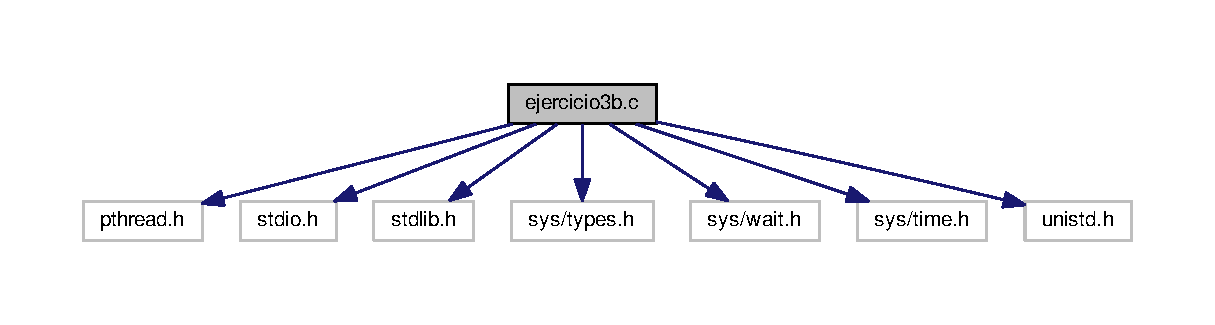
\includegraphics[width=350pt]{ejercicio3b_8c__incl}
\end{center}
\end{figure}
\subsection*{\textquotesingle{}defines\textquotesingle{}}
\begin{DoxyCompactItemize}
\item 
\#define \hyperlink{ejercicio3b_8c_a1541b4eafb644db053370db475c0ea71}{N\+U\+M\+\_\+\+H\+IL}~100
\end{DoxyCompactItemize}
\subsection*{Funciones}
\begin{DoxyCompactItemize}
\item 
void $\ast$ \hyperlink{ejercicio3b_8c_a3c96e5c70f817235701b2e9543215a1d}{is\+\_\+prime} (void $\ast$arg)
\begin{DoxyCompactList}\small\item\em funcion que lista los np primeros primos \end{DoxyCompactList}\item 
int \hyperlink{ejercicio3b_8c_a0ddf1224851353fc92bfbff6f499fa97}{main} (int argc, char $\ast$argv\mbox{[}$\,$\mbox{]})
\begin{DoxyCompactList}\small\item\em funcion de hilos de un proceso \end{DoxyCompactList}\end{DoxyCompactItemize}


\subsection{Descripción detallada}
Implementa el ejercicio 3b de hilos de un proceso. 

\begin{DoxyAuthor}{Autor}
Andres Salas \href{mailto:andres.salas@estudiante.uam.es}{\tt andres.\+salas@estudiante.\+uam.\+es} 

Antonio Martin \href{mailto:antonio.martinmasuda@estudiante.uam.es}{\tt antonio.\+martinmasuda@estudiante.\+uam.\+es} 
\end{DoxyAuthor}
\begin{DoxyNote}{Nota}
Grupo 2202 
\end{DoxyNote}
\begin{DoxyVersion}{Versión}
1.\+0 
\end{DoxyVersion}
\begin{DoxyDate}{Fecha}
03/03/2017 
\end{DoxyDate}


\subsection{Documentación de los \textquotesingle{}defines\textquotesingle{}}
\index{ejercicio3b.\+c@{ejercicio3b.\+c}!N\+U\+M\+\_\+\+H\+IL@{N\+U\+M\+\_\+\+H\+IL}}
\index{N\+U\+M\+\_\+\+H\+IL@{N\+U\+M\+\_\+\+H\+IL}!ejercicio3b.\+c@{ejercicio3b.\+c}}
\subsubsection[{\texorpdfstring{N\+U\+M\+\_\+\+H\+IL}{NUM_HIL}}]{\setlength{\rightskip}{0pt plus 5cm}\#define N\+U\+M\+\_\+\+H\+IL~100}\hypertarget{ejercicio3b_8c_a1541b4eafb644db053370db475c0ea71}{}\label{ejercicio3b_8c_a1541b4eafb644db053370db475c0ea71}
Numero de hilos del bucle for 

\subsection{Documentación de las funciones}
\index{ejercicio3b.\+c@{ejercicio3b.\+c}!is\+\_\+prime@{is\+\_\+prime}}
\index{is\+\_\+prime@{is\+\_\+prime}!ejercicio3b.\+c@{ejercicio3b.\+c}}
\subsubsection[{\texorpdfstring{is\+\_\+prime(void $\ast$arg)}{is_prime(void *arg)}}]{\setlength{\rightskip}{0pt plus 5cm}void$\ast$ is\+\_\+prime (
\begin{DoxyParamCaption}
\item[{void $\ast$}]{arg}
\end{DoxyParamCaption}
)}\hypertarget{ejercicio3b_8c_a3c96e5c70f817235701b2e9543215a1d}{}\label{ejercicio3b_8c_a3c96e5c70f817235701b2e9543215a1d}


funcion que lista los np primeros primos 


\begin{DoxyParams}{Parámetros}
{\em arg} & contiene los parámetros pasados por el hilo \\
\hline
\end{DoxyParams}
\begin{DoxyReturn}{Devuelve}
void$\ast$\+: fin del hilo 
\end{DoxyReturn}
\index{ejercicio3b.\+c@{ejercicio3b.\+c}!main@{main}}
\index{main@{main}!ejercicio3b.\+c@{ejercicio3b.\+c}}
\subsubsection[{\texorpdfstring{main(int argc, char $\ast$argv[])}{main(int argc, char *argv[])}}]{\setlength{\rightskip}{0pt plus 5cm}int main (
\begin{DoxyParamCaption}
\item[{int}]{argc, }
\item[{char $\ast$}]{argv\mbox{[}$\,$\mbox{]}}
\end{DoxyParamCaption}
)}\hypertarget{ejercicio3b_8c_a0ddf1224851353fc92bfbff6f499fa97}{}\label{ejercicio3b_8c_a0ddf1224851353fc92bfbff6f499fa97}


funcion de hilos de un proceso 


\begin{DoxyParams}{Parámetros}
{\em argc} & contiene el número de parámetros totales pasados \\
\hline
{\em argv\mbox{[}$\,$\mbox{]}} & contiene los parámetros pasados por el usuario \\
\hline
\end{DoxyParams}
\begin{DoxyReturn}{Devuelve}
int\+: valor de exito o fracaso 
\end{DoxyReturn}

\hypertarget{ejercicio4a_8c}{}\section{Referencia del Archivo ejercicio4a.\+c}
\label{ejercicio4a_8c}\index{ejercicio4a.\+c@{ejercicio4a.\+c}}


Implementa el ejercicio 4a de multiplicacion de matrices.  


{\ttfamily \#include $<$stdio.\+h$>$}\\*
{\ttfamily \#include $<$stdlib.\+h$>$}\\*
{\ttfamily \#include $<$string.\+h$>$}\\*
{\ttfamily \#include $<$pthread.\+h$>$}\\*
{\ttfamily \#include $<$unistd.\+h$>$}\\*
Dependencia gráfica adjunta para ejercicio4a.\+c\+:\nopagebreak
\begin{figure}[H]
\begin{center}
\leavevmode
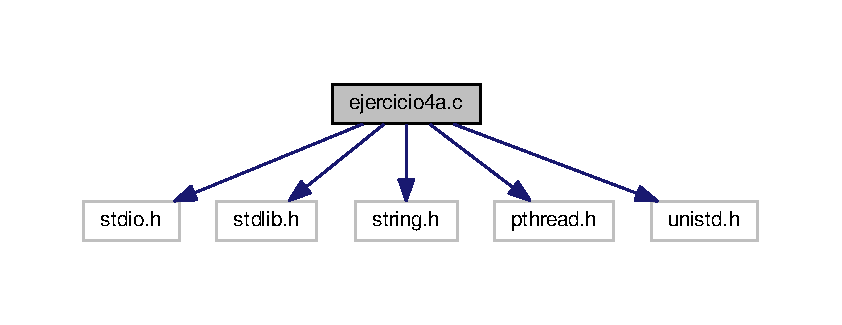
\includegraphics[width=350pt]{ejercicio4a_8c__incl}
\end{center}
\end{figure}
\subsection*{Clases}
\begin{DoxyCompactItemize}
\item 
struct \hyperlink{struct__params}{\+\_\+params}
\begin{DoxyCompactList}\small\item\em Estructura params que contiene los parametros necesarios para que el hilo multiplique un matriz por un numero entero. \end{DoxyCompactList}\end{DoxyCompactItemize}
\subsection*{\textquotesingle{}defines\textquotesingle{}}
\begin{DoxyCompactItemize}
\item 
\#define {\bfseries M\+A\+X\+T\+AM}~256\hypertarget{ejercicio4a_8c_a0e68c4ad6b4b3a349afa80ebbbdffb13}{}\label{ejercicio4a_8c_a0e68c4ad6b4b3a349afa80ebbbdffb13}

\end{DoxyCompactItemize}
\subsection*{\textquotesingle{}typedefs\textquotesingle{}}
\begin{DoxyCompactItemize}
\item 
typedef struct \hyperlink{struct__params}{\+\_\+params} \hyperlink{ejercicio4a_8c_ac8d4b7ef3bb36bb6a956ac657e9a0b8f}{params}\hypertarget{ejercicio4a_8c_ac8d4b7ef3bb36bb6a956ac657e9a0b8f}{}\label{ejercicio4a_8c_ac8d4b7ef3bb36bb6a956ac657e9a0b8f}

\begin{DoxyCompactList}\small\item\em Estructura params que contiene los parametros necesarios para que el hilo multiplique un matriz por un numero entero. \end{DoxyCompactList}\end{DoxyCompactItemize}
\subsection*{Funciones}
\begin{DoxyCompactItemize}
\item 
int \hyperlink{ejercicio4a_8c_af2eaee395141f1e236459336cbf0fdee}{comprueba\+\_\+matriz} (char $\ast$aux, int dim, int $\ast$matriz)
\begin{DoxyCompactList}\small\item\em funcion que comprueba si la matriz introducida por el usuario es valida \end{DoxyCompactList}\item 
void $\ast$ \hyperlink{ejercicio4a_8c_ae04da77ba1f41c03d3f8a0f19797333f}{multiplicacion} (void $\ast$arg)
\begin{DoxyCompactList}\small\item\em funcion que multiplica una matriz por un escalar \end{DoxyCompactList}\item 
int \hyperlink{ejercicio4a_8c_ae66f6b31b5ad750f1fe042a706a4e3d4}{main} ()
\begin{DoxyCompactList}\small\item\em funcion que implementa la multiplicacion de matriz por escalar mediante dos hilos \end{DoxyCompactList}\end{DoxyCompactItemize}


\subsection{Descripción detallada}
Implementa el ejercicio 4a de multiplicacion de matrices. 

\begin{DoxyAuthor}{Autor}
Andres Salas \href{mailto:andres.salas@estudiante.uam.es}{\tt andres.\+salas@estudiante.\+uam.\+es} 

Antonio Martin \href{mailto:antonio.martinmasuda@estudiante.uam.es}{\tt antonio.\+martinmasuda@estudiante.\+uam.\+es} 
\end{DoxyAuthor}
\begin{DoxyNote}{Nota}
Grupo 2202 
\end{DoxyNote}
\begin{DoxyVersion}{Versión}
1.\+0 
\end{DoxyVersion}
\begin{DoxyDate}{Fecha}
04/03/2017 
\end{DoxyDate}


\subsection{Documentación de las funciones}
\index{ejercicio4a.\+c@{ejercicio4a.\+c}!comprueba\+\_\+matriz@{comprueba\+\_\+matriz}}
\index{comprueba\+\_\+matriz@{comprueba\+\_\+matriz}!ejercicio4a.\+c@{ejercicio4a.\+c}}
\subsubsection[{\texorpdfstring{comprueba\+\_\+matriz(char $\ast$aux, int dim, int $\ast$matriz)}{comprueba_matriz(char *aux, int dim, int *matriz)}}]{\setlength{\rightskip}{0pt plus 5cm}int comprueba\+\_\+matriz (
\begin{DoxyParamCaption}
\item[{char $\ast$}]{aux, }
\item[{int}]{dim, }
\item[{int $\ast$}]{matriz}
\end{DoxyParamCaption}
)}\hypertarget{ejercicio4a_8c_af2eaee395141f1e236459336cbf0fdee}{}\label{ejercicio4a_8c_af2eaee395141f1e236459336cbf0fdee}


funcion que comprueba si la matriz introducida por el usuario es valida 


\begin{DoxyParams}{Parámetros}
{\em aux} & cadena de caracteres que ha introducido el usuario \\
\hline
{\em dim} & dimension de la matriz \\
\hline
{\em matriz} & array donde se almacenaran los enteros introducidos por el usuario si la matriz es valida \\
\hline
\end{DoxyParams}
\begin{DoxyReturn}{Devuelve}
int\+: E\+X\+I\+T\+\_\+\+S\+U\+C\+C\+E\+SS en caso de que la matriz es valida o E\+X\+I\+T\+\_\+\+F\+A\+I\+L\+U\+RE en caso de que no se hayan introducido suficientes numeros o haya introducido caracteres no numericos 
\end{DoxyReturn}
\index{ejercicio4a.\+c@{ejercicio4a.\+c}!main@{main}}
\index{main@{main}!ejercicio4a.\+c@{ejercicio4a.\+c}}
\subsubsection[{\texorpdfstring{main()}{main()}}]{\setlength{\rightskip}{0pt plus 5cm}int main (
\begin{DoxyParamCaption}
{}
\end{DoxyParamCaption}
)}\hypertarget{ejercicio4a_8c_ae66f6b31b5ad750f1fe042a706a4e3d4}{}\label{ejercicio4a_8c_ae66f6b31b5ad750f1fe042a706a4e3d4}


funcion que implementa la multiplicacion de matriz por escalar mediante dos hilos 

\begin{DoxyReturn}{Devuelve}
int\+: valor de exito o fracaso 
\end{DoxyReturn}
\index{ejercicio4a.\+c@{ejercicio4a.\+c}!multiplicacion@{multiplicacion}}
\index{multiplicacion@{multiplicacion}!ejercicio4a.\+c@{ejercicio4a.\+c}}
\subsubsection[{\texorpdfstring{multiplicacion(void $\ast$arg)}{multiplicacion(void *arg)}}]{\setlength{\rightskip}{0pt plus 5cm}void$\ast$ multiplicacion (
\begin{DoxyParamCaption}
\item[{void $\ast$}]{arg}
\end{DoxyParamCaption}
)}\hypertarget{ejercicio4a_8c_ae04da77ba1f41c03d3f8a0f19797333f}{}\label{ejercicio4a_8c_ae04da77ba1f41c03d3f8a0f19797333f}


funcion que multiplica una matriz por un escalar 


\begin{DoxyParams}{Parámetros}
{\em arg} & se le pasara la estructura de hilos \\
\hline
\end{DoxyParams}
\begin{DoxyReturn}{Devuelve}
void$\ast$\+: finaliza la funcion con la salida del hilo 
\end{DoxyReturn}

\hypertarget{ejercicio4b_8c}{}\section{Referencia del Archivo ejercicio4b.\+c}
\label{ejercicio4b_8c}\index{ejercicio4b.\+c@{ejercicio4b.\+c}}


Implementa el ejercicio 4b de multiplicacion de matrices.  


{\ttfamily \#include $<$stdio.\+h$>$}\\*
{\ttfamily \#include $<$stdlib.\+h$>$}\\*
{\ttfamily \#include $<$string.\+h$>$}\\*
{\ttfamily \#include $<$pthread.\+h$>$}\\*
{\ttfamily \#include $<$unistd.\+h$>$}\\*
Dependencia gráfica adjunta para ejercicio4b.\+c\+:\nopagebreak
\begin{figure}[H]
\begin{center}
\leavevmode
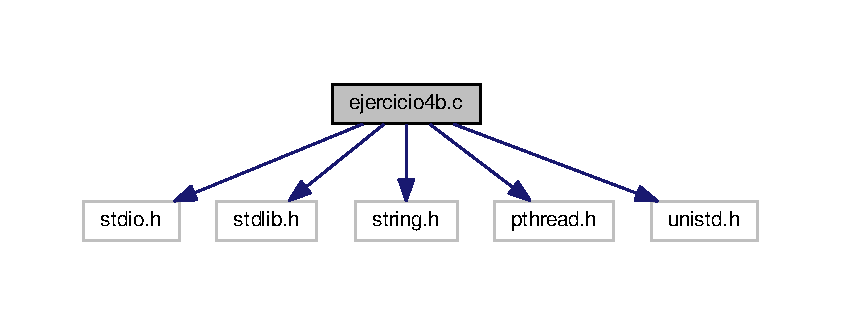
\includegraphics[width=350pt]{ejercicio4b_8c__incl}
\end{center}
\end{figure}
\subsection*{Clases}
\begin{DoxyCompactItemize}
\item 
struct \hyperlink{struct__params}{\+\_\+params}
\begin{DoxyCompactList}\small\item\em Estructura params que contiene los parametros necesarios para que el hilo multiplique un matriz por un numero entero. \end{DoxyCompactList}\end{DoxyCompactItemize}
\subsection*{\textquotesingle{}defines\textquotesingle{}}
\begin{DoxyCompactItemize}
\item 
\#define \hyperlink{ejercicio4b_8c_a0e68c4ad6b4b3a349afa80ebbbdffb13}{M\+A\+X\+T\+AM}~256 /$\ast$tamanyo maximo$\ast$/\hypertarget{ejercicio4b_8c_a0e68c4ad6b4b3a349afa80ebbbdffb13}{}\label{ejercicio4b_8c_a0e68c4ad6b4b3a349afa80ebbbdffb13}

\begin{DoxyCompactList}\small\item\em Definicion de la macro M\+A\+X\+T\+AM. \end{DoxyCompactList}\end{DoxyCompactItemize}
\subsection*{\textquotesingle{}typedefs\textquotesingle{}}
\begin{DoxyCompactItemize}
\item 
typedef struct \hyperlink{struct__params}{\+\_\+params} \hyperlink{ejercicio4b_8c_ac8d4b7ef3bb36bb6a956ac657e9a0b8f}{params}\hypertarget{ejercicio4b_8c_ac8d4b7ef3bb36bb6a956ac657e9a0b8f}{}\label{ejercicio4b_8c_ac8d4b7ef3bb36bb6a956ac657e9a0b8f}

\begin{DoxyCompactList}\small\item\em Estructura params que contiene los parametros necesarios para que el hilo multiplique un matriz por un numero entero. Se ha incluido un puntero a la propia estructura que apuntara a la estructura del otro hilo. \end{DoxyCompactList}\end{DoxyCompactItemize}
\subsection*{Funciones}
\begin{DoxyCompactItemize}
\item 
int \hyperlink{ejercicio4b_8c_af2eaee395141f1e236459336cbf0fdee}{comprueba\+\_\+matriz} (char $\ast$aux, int dim, int $\ast$matriz)
\begin{DoxyCompactList}\small\item\em funcion que comprueba si la matriz introducida por el usuario es valida \end{DoxyCompactList}\item 
void $\ast$ \hyperlink{ejercicio4b_8c_ae04da77ba1f41c03d3f8a0f19797333f}{multiplicacion} (void $\ast$arg)
\begin{DoxyCompactList}\small\item\em funcion que multiplica una matriz por un escalar \end{DoxyCompactList}\item 
int \hyperlink{ejercicio4b_8c_ae66f6b31b5ad750f1fe042a706a4e3d4}{main} ()
\begin{DoxyCompactList}\small\item\em funcion que implementa la multiplicacion de matriz por escalar mediante dos hilos \end{DoxyCompactList}\end{DoxyCompactItemize}


\subsection{Descripción detallada}
Implementa el ejercicio 4b de multiplicacion de matrices. 

\begin{DoxyAuthor}{Autor}
Andres Salas \href{mailto:andres.salas@estudiante.uam.es}{\tt andres.\+salas@estudiante.\+uam.\+es} 

Antonio Martin \href{mailto:antonio.martinmasuda@estudiante.uam.es}{\tt antonio.\+martinmasuda@estudiante.\+uam.\+es} 
\end{DoxyAuthor}
\begin{DoxyNote}{Nota}
Grupo 2202 
\end{DoxyNote}
\begin{DoxyVersion}{Versión}
1.\+0 
\end{DoxyVersion}
\begin{DoxyDate}{Fecha}
04/03/2017 
\end{DoxyDate}


\subsection{Documentación de las funciones}
\index{ejercicio4b.\+c@{ejercicio4b.\+c}!comprueba\+\_\+matriz@{comprueba\+\_\+matriz}}
\index{comprueba\+\_\+matriz@{comprueba\+\_\+matriz}!ejercicio4b.\+c@{ejercicio4b.\+c}}
\subsubsection[{\texorpdfstring{comprueba\+\_\+matriz(char $\ast$aux, int dim, int $\ast$matriz)}{comprueba_matriz(char *aux, int dim, int *matriz)}}]{\setlength{\rightskip}{0pt plus 5cm}int comprueba\+\_\+matriz (
\begin{DoxyParamCaption}
\item[{char $\ast$}]{aux, }
\item[{int}]{dim, }
\item[{int $\ast$}]{matriz}
\end{DoxyParamCaption}
)}\hypertarget{ejercicio4b_8c_af2eaee395141f1e236459336cbf0fdee}{}\label{ejercicio4b_8c_af2eaee395141f1e236459336cbf0fdee}


funcion que comprueba si la matriz introducida por el usuario es valida 


\begin{DoxyParams}{Parámetros}
{\em aux} & cadena de caracteres que ha introducido el usuario \\
\hline
{\em dim} & dimension de la matriz \\
\hline
{\em matriz} & array donde se almacenaran los enteros introducidos por el usuario si la matriz es valida \\
\hline
\end{DoxyParams}
\begin{DoxyReturn}{Devuelve}
int\+: E\+X\+I\+T\+\_\+\+S\+U\+C\+C\+E\+SS en caso de que la matriz es valida o E\+X\+I\+T\+\_\+\+F\+A\+I\+L\+U\+RE en caso de que no se hayan introducido suficientes numeros o haya introducido caracteres no numericos 
\end{DoxyReturn}
\index{ejercicio4b.\+c@{ejercicio4b.\+c}!main@{main}}
\index{main@{main}!ejercicio4b.\+c@{ejercicio4b.\+c}}
\subsubsection[{\texorpdfstring{main()}{main()}}]{\setlength{\rightskip}{0pt plus 5cm}int main (
\begin{DoxyParamCaption}
{}
\end{DoxyParamCaption}
)}\hypertarget{ejercicio4b_8c_ae66f6b31b5ad750f1fe042a706a4e3d4}{}\label{ejercicio4b_8c_ae66f6b31b5ad750f1fe042a706a4e3d4}


funcion que implementa la multiplicacion de matriz por escalar mediante dos hilos 

\begin{DoxyReturn}{Devuelve}
int\+: valor de exito o fracaso 
\end{DoxyReturn}
\index{ejercicio4b.\+c@{ejercicio4b.\+c}!multiplicacion@{multiplicacion}}
\index{multiplicacion@{multiplicacion}!ejercicio4b.\+c@{ejercicio4b.\+c}}
\subsubsection[{\texorpdfstring{multiplicacion(void $\ast$arg)}{multiplicacion(void *arg)}}]{\setlength{\rightskip}{0pt plus 5cm}void$\ast$ multiplicacion (
\begin{DoxyParamCaption}
\item[{void $\ast$}]{arg}
\end{DoxyParamCaption}
)}\hypertarget{ejercicio4b_8c_ae04da77ba1f41c03d3f8a0f19797333f}{}\label{ejercicio4b_8c_ae04da77ba1f41c03d3f8a0f19797333f}


funcion que multiplica una matriz por un escalar 


\begin{DoxyParams}{Parámetros}
{\em arg} & se le pasara la estructura de hilos \\
\hline
\end{DoxyParams}
\begin{DoxyReturn}{Devuelve}
void$\ast$\+: finaliza la funcion con la salida del hilo 
\end{DoxyReturn}

\hypertarget{ejercicio6_8c}{}\section{Referencia del Archivo ejercicio6.\+c}
\label{ejercicio6_8c}\index{ejercicio6.\+c@{ejercicio6.\+c}}


Implementa el ejercicio 6 de relacion entre procesos padre/hijo.  


{\ttfamily \#include $<$stdio.\+h$>$}\\*
{\ttfamily \#include $<$stdlib.\+h$>$}\\*
{\ttfamily \#include $<$sys/types.\+h$>$}\\*
{\ttfamily \#include $<$sys/wait.\+h$>$}\\*
{\ttfamily \#include $<$unistd.\+h$>$}\\*
Dependencia gráfica adjunta para ejercicio6.\+c\+:\nopagebreak
\begin{figure}[H]
\begin{center}
\leavevmode
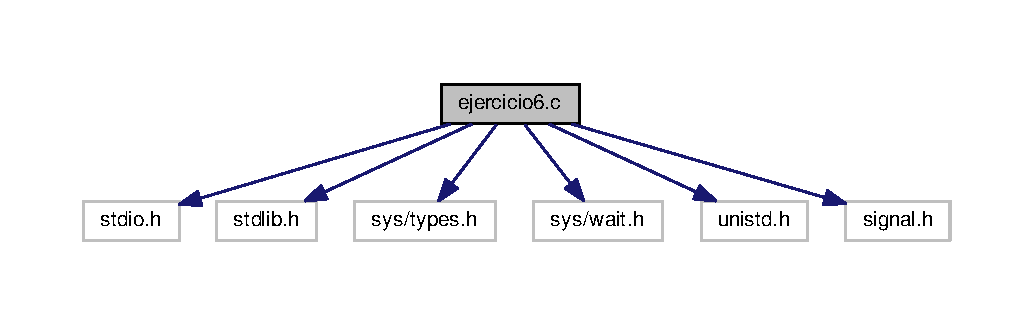
\includegraphics[width=350pt]{ejercicio6_8c__incl}
\end{center}
\end{figure}
\subsection*{\textquotesingle{}defines\textquotesingle{}}
\begin{DoxyCompactItemize}
\item 
\#define \hyperlink{ejercicio6_8c_a4cc8fa399feaab01926e82767a97a96b}{C\+A\+D\+E\+NA}~80
\end{DoxyCompactItemize}
\subsection*{Funciones}
\begin{DoxyCompactItemize}
\item 
int \hyperlink{ejercicio6_8c_a840291bc02cba5474a4cb46a9b9566fe}{main} (void)
\begin{DoxyCompactList}\small\item\em funcion en la que el proceso padre reserva memoria y en el proceso hijo el usuario introduce un nombre \end{DoxyCompactList}\end{DoxyCompactItemize}


\subsection{Descripción detallada}
Implementa el ejercicio 6 de relacion entre procesos padre/hijo. 

\begin{DoxyAuthor}{Autor}
Andres Salas \href{mailto:andres.salas@estudiante.uam.es}{\tt andres.\+salas@estudiante.\+uam.\+es} 

Antonio Martin \href{mailto:antonio.martinmasuda@estudiante.uam.es}{\tt antonio.\+martinmasuda@estudiante.\+uam.\+es} 
\end{DoxyAuthor}
\begin{DoxyNote}{Nota}
Grupo 2202 
\end{DoxyNote}
\begin{DoxyVersion}{Versión}
1.\+0 
\end{DoxyVersion}
\begin{DoxyDate}{Fecha}
10/02/2017 
\end{DoxyDate}


\subsection{Documentación de los \textquotesingle{}defines\textquotesingle{}}
\index{ejercicio6.\+c@{ejercicio6.\+c}!C\+A\+D\+E\+NA@{C\+A\+D\+E\+NA}}
\index{C\+A\+D\+E\+NA@{C\+A\+D\+E\+NA}!ejercicio6.\+c@{ejercicio6.\+c}}
\subsubsection[{\texorpdfstring{C\+A\+D\+E\+NA}{CADENA}}]{\setlength{\rightskip}{0pt plus 5cm}\#define C\+A\+D\+E\+NA~80}\hypertarget{ejercicio6_8c_a4cc8fa399feaab01926e82767a97a96b}{}\label{ejercicio6_8c_a4cc8fa399feaab01926e82767a97a96b}
Numero de caracteres de la cadena 

\subsection{Documentación de las funciones}
\index{ejercicio6.\+c@{ejercicio6.\+c}!main@{main}}
\index{main@{main}!ejercicio6.\+c@{ejercicio6.\+c}}
\subsubsection[{\texorpdfstring{main(void)}{main(void)}}]{\setlength{\rightskip}{0pt plus 5cm}int main (
\begin{DoxyParamCaption}
\item[{void}]{}
\end{DoxyParamCaption}
)}\hypertarget{ejercicio6_8c_a840291bc02cba5474a4cb46a9b9566fe}{}\label{ejercicio6_8c_a840291bc02cba5474a4cb46a9b9566fe}


funcion en la que el proceso padre reserva memoria y en el proceso hijo el usuario introduce un nombre 

\begin{DoxyReturn}{Devuelve}
int\+: valor de exito o fracaso 
\end{DoxyReturn}

%--- End generated contents ---

% Index
\backmatter
\newpage
\phantomsection
\clearemptydoublepage
\addcontentsline{toc}{chapter}{Índice}
\printindex

\end{document}
